% English draft based on sections/04_response_channels_ja.tex
\section{Response Channels and Silent Worlds}

\noindent\textbf{Scope of the account.} Responsive and silent retain their nonontological, model-local distinction. Their boundary is a candidate relation, not a calibrated threshold. The regress argument is conditional on its three stated premises; it does not establish the occurrence of psychological divergence. Branching and regress are role analogies. Trace retention, recursive use, and emergence of a stopping layer are distinct processes: none is established simply by naming traces as logs or by assuming nonclosure.


The historical local-state account in \S{}3 discussed a conditional fixed-point model for $L_F$, not an unrestricted cognitive stopping theorem. This chapter asks how that non-closure appears in different operating environments. The distinction between responsive and silent worlds is not ontological. It is a threshold phenomenon.

\subsection{Responsive and Silent Regimes}

A responsive world is an environment in which an inferential output receives a return. The agent asks, acts, hypothesizes, or experiments, and the world responds. In C-geometry, the gradient forms a closed loop: the output changes the world, and the changed world returns as feedback.

A silent world is an environment in which such return does not close. The agent can output inference, but no corresponding response comes back. Ultimate reasons, fixed past events, and unresolved future contingencies often appear in this mode.

Formally, a responsive regime has significant mutual constraint in both directions, $H_{ij}$ and $H_{ji}$. A silent regime has a broken or negligible return channel, approximately $H_{ji}\approx 0$.

\subsection{Silence Is Not Defect}

Silence is not a defect in the world. It is not merely ignorance waiting to be solved. Some regions do not return the kind of response required to close the inferential loop. If responsive-world strategies are applied to silent-world regions without threshold mobility, inference can enter infinite regress.

\subsection{Threshold Phenomenon}

Responsive and silent regimes are phases determined by thresholds. The same environment can appear responsive or silent depending on the position of the boundary set by parameters such as inferential velocity, resolution, and stopping hardness. The threshold mobility $\mu_\theta$ is the ability to move this boundary.

\begin{figure}[H]
\centering
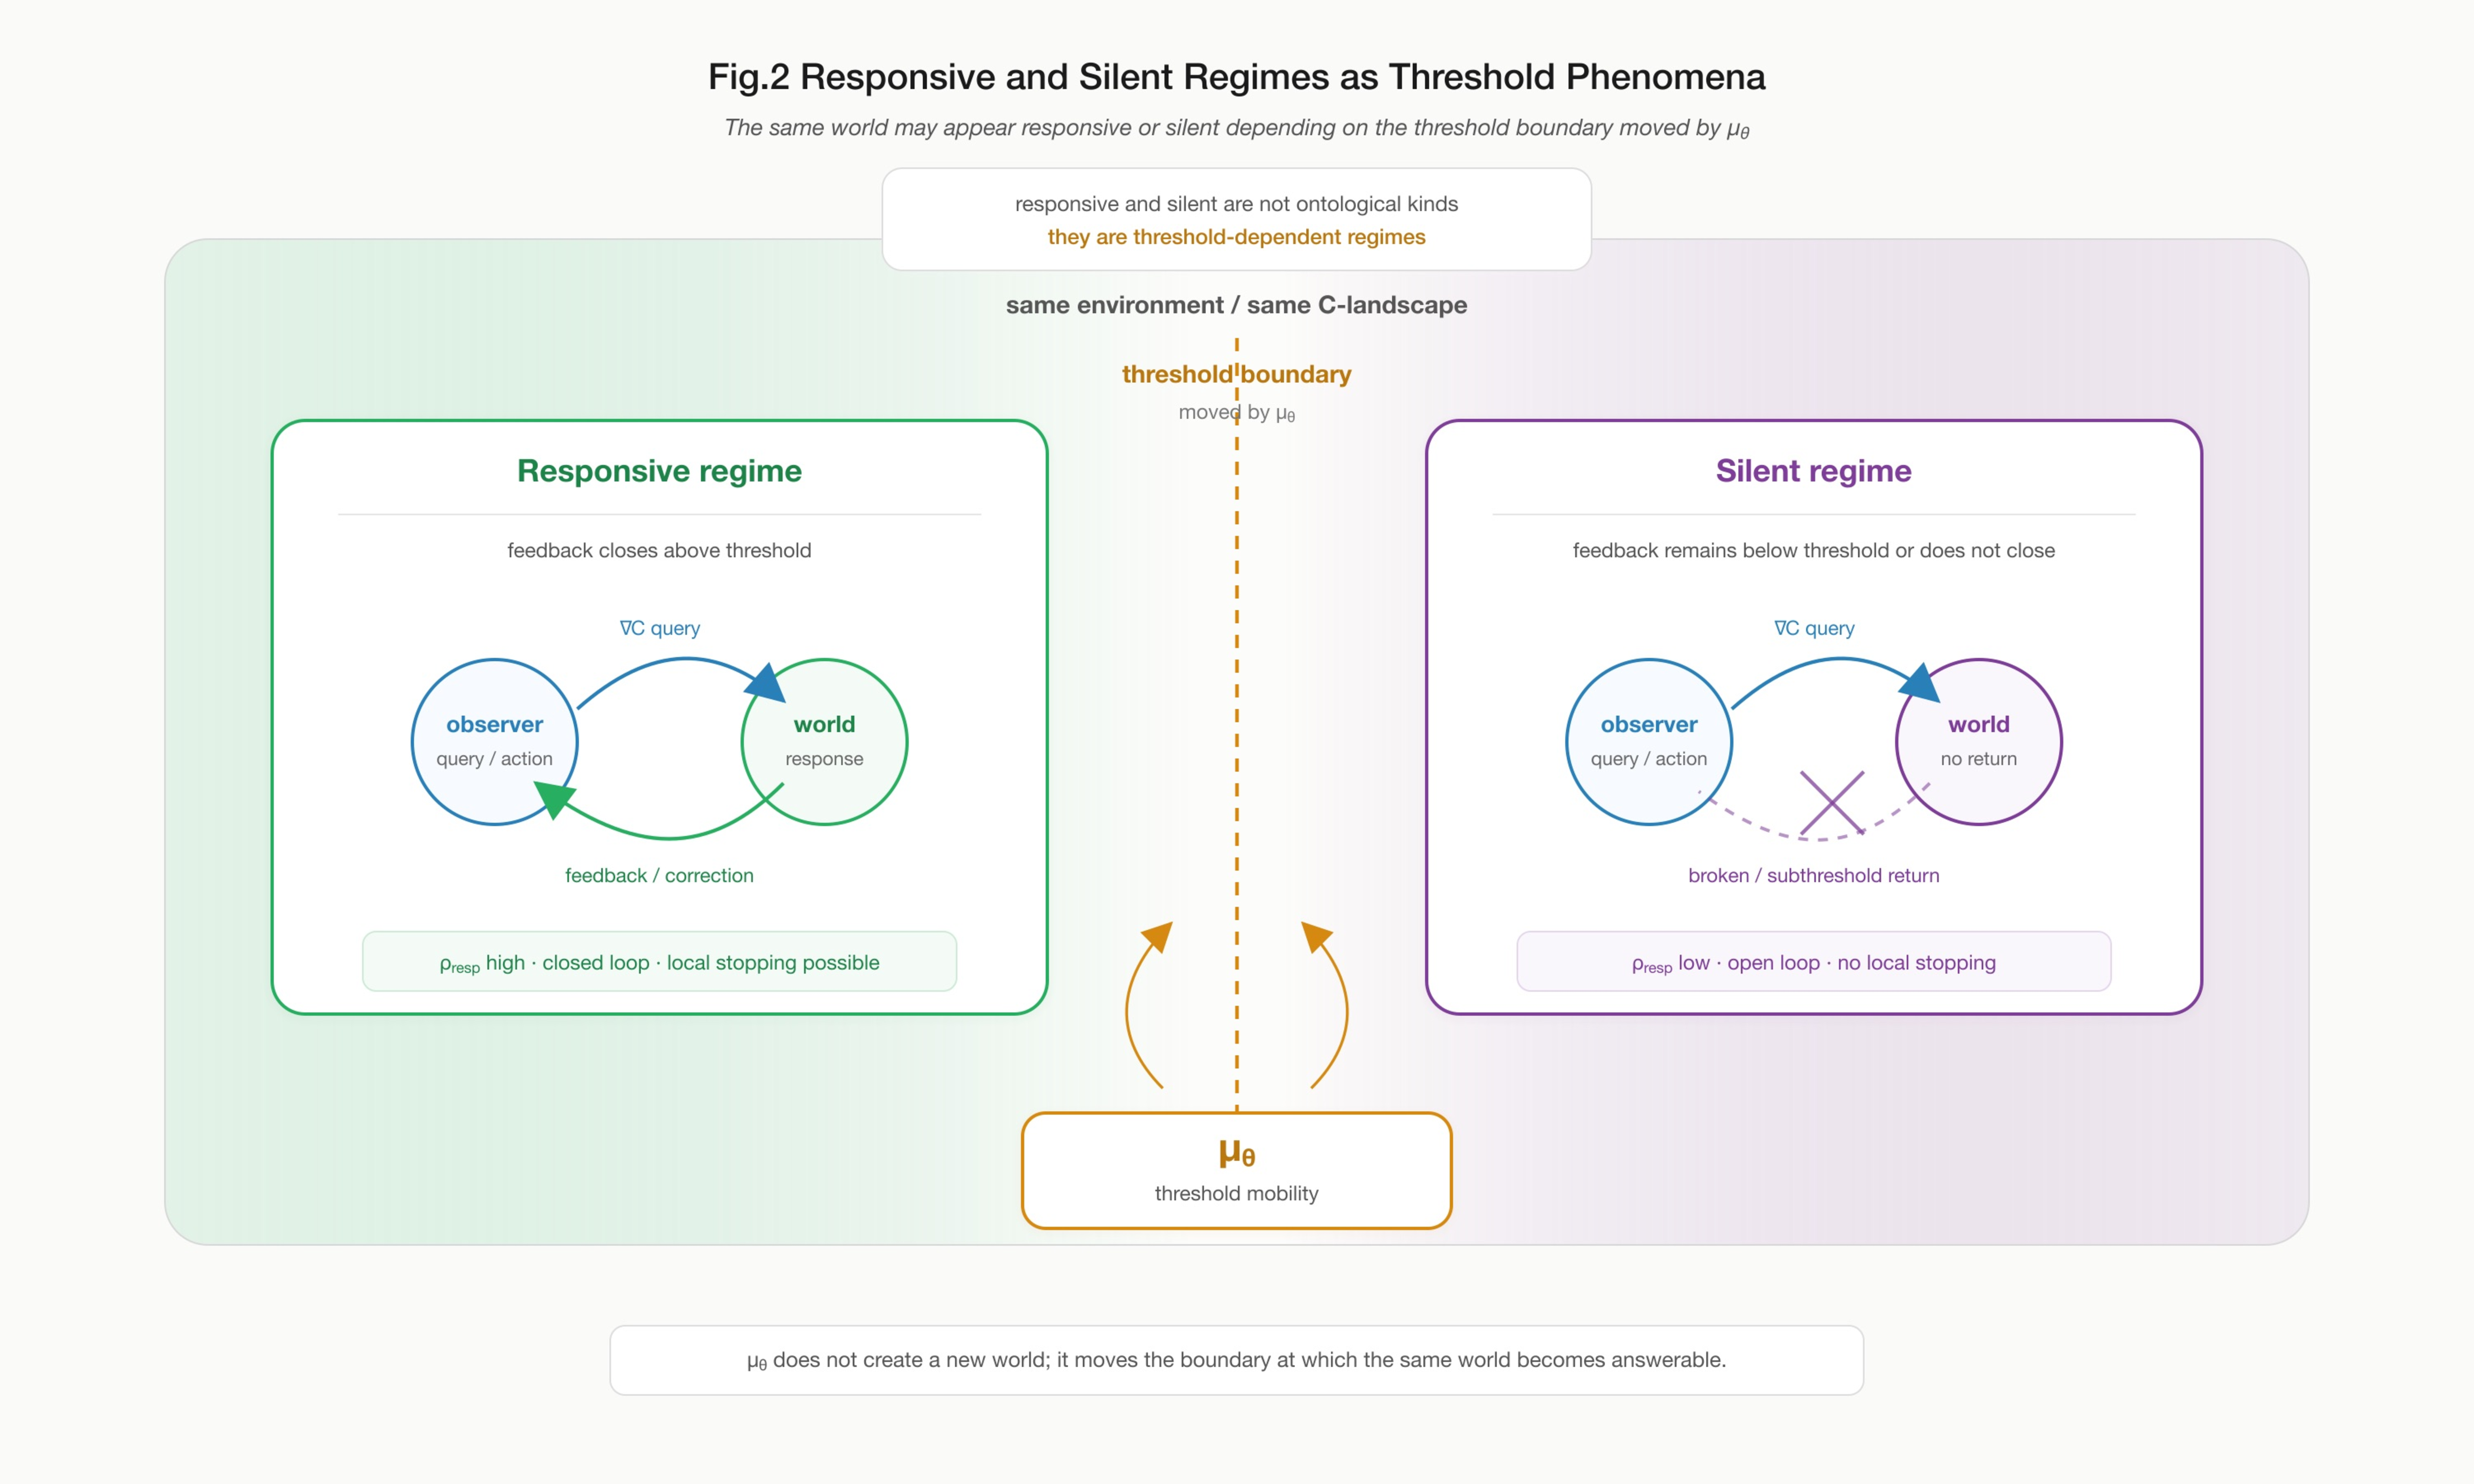
\includegraphics[width=\linewidth]{fig2_responsive_silent_threshold.pdf}
\caption{Responsive and silent regimes. These are not two ontological kinds of world, but threshold-dependent phases determined by the boundary moved by $\mu_\theta$.}
\label{fig:part2-responsive-silent}
\figurenote{Both panels compare one environment and a model-local C-landscape under different proposed threshold boundaries.}{External mutual constraint and local stopping are related as a functional hypothesis. The diagram does not derive cognitive stopping or the necessity of externalization.}
\end{figure}

\subsection{Infinite Regress in Silent Worlds}

For the historical local-state regress model, assume the three stated conditions: no stopping response, justification advanced by inference, and no stopping resource specified within that inference. Continued reapplication then describes a nonterminating model. A silent-regime label does not independently establish these premises for cognition.

In that historical discussion, infinite regress, absence of a fixed point, and branching growth are distinct descriptions. Their combination as cognitive instability is a hypothesis, not a result established by silence or non-fixedness alone.

\subsection{The Preview of $L_R$}

For the preview and closing discussion below, retained traces are candidates for recursive use, not an automatic result of continued inference. The active LR role and temporary scaffold account are specified in Section 5, separately from a process of reference. The preserved regress-to-layer chain motivates a historical hypothesis, not support identity, access, or LE formation.

Traces of inference are called logs when retained in the proposed account. A layer of recursive reference to them is named $L_R$. Neither retention nor actual recursive access follows merely from continuing inference.

This is the bridge to \S{}5. The historical model's failure of $L_F$ to stop is not only a dead end. It motivates a hypothesis: retained traces may support recursive reference, and $L_E$ is proposed in relation to that reference and external constraint. Neither retention nor emergence follows from nonclosure alone.

\bigskip
